\documentclass{beamer}
%
% Choose how your presentation looks.
%
% For more themes, color themes and font themes, see:
% http://deic.uab.es/~iblanes/beamer_gallery/index_by_theme.html
%
\mode<presentation>
{
  \usetheme{Boadilla}      % or try Darmstadt, Madrid, Warsaw, ...
  \usecolortheme{beaver} % or try albatross, beaver, crane, ...
  \usefonttheme{default}  % or try serif, structurebold, ...
  \setbeamertemplate{navigation symbols}{}
  \setbeamertemplate{caption}[numbered]
  
} 

\usepackage{xcolor,colortbl}
\usepackage[english]{babel}
\usepackage[utf8x]{inputenc}
\usepackage{courier}
\usepackage{dsfont}
\usepackage{verbatim} 
\usepackage{enumerate}
\usepackage{tikz}
\usepackage{multirow}
\usepackage{venndiagram}
\usepackage{epigraph} 
%\usepackage{xcolor}
\usepackage{makecell}

%\usepackage{enumitem}

\usepackage{hyperref}
\hypersetup{
    colorlinks=true,
    linkcolor=blue,
    filecolor=magenta,      
    urlcolor=cyan,
}

% R stuff!
\usepackage{listings}
\definecolor{codegreen}{rgb}{0,0.6,0}
\definecolor{codegray}{rgb}{0.5,0.5,0.5}
\definecolor{codepurple}{rgb}{0.58,0,0.82}
\definecolor{backcolour}{rgb}{0.95,0.95,0.92}

\lstdefinestyle{mystyle}{
    backgroundcolor=\color{backcolour},    
    commentstyle=\color{codegreen},
    keywordstyle=\color{black},
    numberstyle=\tiny\color{codegray},
    stringstyle=\color{codepurple},
    basicstyle=\ttfamily\footnotesize,
    breakatwhitespace=false,         
    breaklines=true,                 
    captionpos=b,                    
    keepspaces=true,                 
    numbers=left,                    
    numbersep=5pt,                  
    showspaces=false,                
    showstringspaces=false,
    showtabs=false,                  
    tabsize=2
}

\lstset{style=mystyle}


\setbeamertemplate{enumerate items}[default]
\setbeamertemplate{itemize item}[triangle]

%\setitemize{label=\usebeamerfont*{itemize item}%
%  \usebeamercolor[fg]{itemize item}
%  \usebeamertemplate{itemize item}}



\title[Introduction to Statistics]{Confidence Intervals}
\subtitle{What can we do with Standard Error?}
\author{Grinnell College}
\date{}

\graphicspath{{img/}}

\begin{document}

\begin{frame}
  \titlepage
\end{frame}

\begin{frame}{Review}
Normal distribution
\begin{itemize}
    \item unimodal + symmetric bell-curve
    \item probabilities
\end{itemize} \vspace{6mm}

Central Limit Theorem:
\begin{enumerate}
    \item If variable X has mean $\mu$ and std.dev. $\sigma$, and
    \item If the number of observations in the sample (n) is large
    \item then the sampling distribution for $\overline{X}$ (sample mean) is Normal with mean $\mu$ and standard error $\sigma / \sqrt{n}$.
\end{enumerate}
\begin{center}
    $\overline{X} \sim$ N($\mu$, $\sigma^2 / n$)
\end{center}
\end{frame}

\begin{frame}{Review -- Sources of Variation}
\textbf{Pop. Standard Deviation:} Description of the variability in our \textit{population}. It is often denoted \textbf{$\sigma$} \vspace{8mm}

\textbf{Sample Standard Deviation:} Description of the variability in our \textit{observations} (sample). It is often denoted \textbf{s} \vspace{8mm}

\textbf{Standard Error: } Description of variability in our \textit{estimates} of a parameter (such as the mean). We will denote standard error as $SE$, with $SE = \sigma / \sqrt{n}$, where $n$ is the number of observations in our sample
\end{frame}

\begin{frame}{Outline}
We saw that the statistic is not going to be exactly equal to the parameter
\begin{itemize}
    \item sampling bias
    \item sampling variability
\end{itemize} \vspace{6mm}

So... we can't just provide a single value for our estimate of the parameter
\begin{itemize}
    \item We also need to quantify how far away our guess is
\end{itemize} \vspace{6mm}

This is why we came up with the \textit{standard error (SE)}, now we need to figure out how to use it. \vspace{6mm}

\textbf{Goal:} We are going to spend today learning how to estimate population means
\end{frame}

\begin{frame}{Example -- COVID Vaccines}
According to the U.S. Census Bureau, as of October 11, 2021: \vspace{2mm}

"83.3\% (+/- 0.5\%) of U.S. adults 18 years and older have received at least one dose of a COVID-19 vaccine.” This is based on a representative sample of civilians aged 18 and over. “Margins of error shown at 90\% confidence.”
\vspace{10mm}

What does margin of error mean?
\end{frame}

\begin{frame}{Intervals}
For the rest of these slides, our goal is to determine the mean of a \textit{population}. \vspace{12mm}

We cannot rely on only our \textbf{point estimate} $\overline{X}$, but perhaps we can find a range of reasonable values that looks like:


\begin{align*}
\text{Point Estimate} \pm \text{Margin of Error}
\end{align*}
\end{frame}

\begin{frame}{A good place to start:}
\begin{center}
    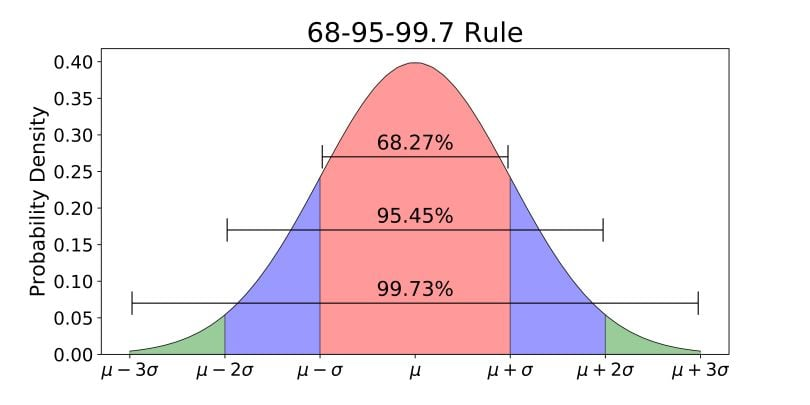
\includegraphics[scale=.45]{img/empirical_rule.jpg}
\end{center}
\end{frame}

\begin{frame}{Good place to start:}
The sampling distribution for the sample mean looks N($\mu$, $\sigma^2 / n$)
\begin{itemize}
    \item Central Limit Theorem
\end{itemize}
\begin{center}
    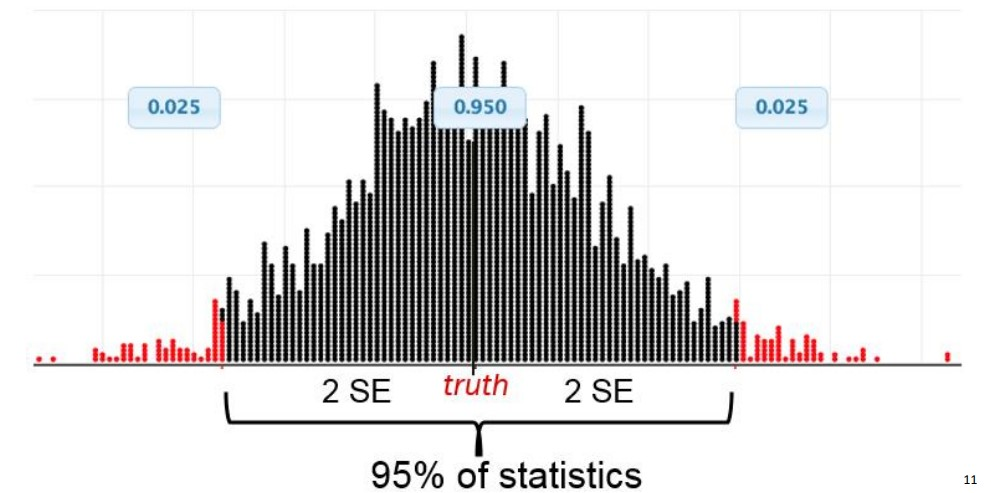
\includegraphics[scale=.57]{img/sampling_dist_CI.jpg}
\end{center}
In the sampling distribution, 95\% of statistics will be within $2 \times$SE of the pop. mean $\mu$
\end{frame}

\begin{frame}{Good place to start:}
The sampling distribution for the sample mean looks N($\mu$, $\sigma^2 / n$)
\begin{itemize}
    \item Central Limit Theorem
\end{itemize}
\begin{center}
    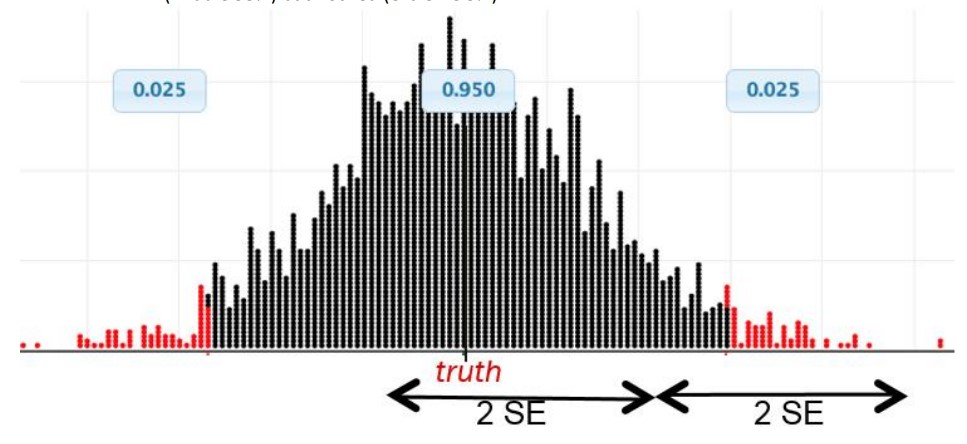
\includegraphics[scale=.57]{img/sampling_dist_CI2.jpg}
\end{center}
Equivalently: The interval 'statistic $\pm$ 
$2\times$SE' will contain $\mu$ for 95\% of the statistics
\end{frame}

\begin{frame}{Confidence Interval}
We are going to call this interval a "95\% Confidence Interval":
\begin{itemize}
    \item 95\% comes from the fact that 95\% of statistics are within 2SE's of the mean
    \item Confidence refers to the fact that this is a range of plausible values for the parameter
\end{itemize} \vspace{10mm}

Formula for a 95\% confidence interval for estimating a pop. mean ($\mu$) is:
\begin{align*}
\overline{x} \pm 2 \times \text{SE}
\end{align*}
\end{frame}

\begin{frame}{Confidence Interval}
Formula for a 95\% confidence interval for estimating a pop. mean ($\mu$) is:
\begin{align*}
\overline{x} \pm 2 \times \text{SE}
\end{align*} \vspace{2mm}


\textbf{Margin of Error} tells us how wide our interval is.
\begin{itemize}
    \item ME = half the width (or length) of the interval
    \item for 95\% CI $\rightarrow$ ME = 2
    $\times$ SE = 2$\frac{\sigma}{\sqrt{n}}$
\end{itemize} \vspace{8mm}

This makes our (final) formula for a 95\% confidence interval for estimating a pop. mean ($\mu$):
\begin{align*}
\overline{x} \pm 2 \times \frac{\sigma}{\sqrt{n}}
\end{align*} \vspace{4mm}
\end{frame}

\begin{frame}{CI Interpretation}
Remember our goal: we are trying to estimate the \textit{population mean} \vspace{6mm}

\textbf{Confidence Interval Interpretation}
\begin{itemize}
    \item mention confidence level
    \item specify the values we got
    \item use context for the population mean when able
\end{itemize} \vspace{6mm}

"We are 95\% confident that (the population mean) is between (lower value) and (upper value)."
\end{frame}

\begin{frame}{Example -- Movie Budgets}
Hollywood movie budget data: $\mu$ = 51.38, $\sigma$ = 57.93 \vspace{2mm}

From a sample of 50 movies we find $\overline{x}$ = 51.01. \vspace{2mm} 

Construct a 95\% Confidence Interval for the pop. mean movie budget. 
\vspace{30mm}
\end{frame}

\begin{frame}{Example -- Movie Budgets}
Hollywood movie budget data: $\mu$ = 51.38, $\sigma$ = 57.93 \vspace{2mm}

From a sample of 50 movies we find $\overline{x}$ = 45.65. \vspace{2mm} 

Construct a 95\% Confidence Interval for the pop. mean movie budget. 
\begin{itemize}
    \item When we know $\sigma$ we can use the formula directly
\end{itemize} \vspace{4mm}
\begin{align*}
    \overline{x} \pm 2\frac{\sigma}{\sqrt{n}} \hspace{2mm}\rightarrow \hspace{2mm} 45.65 \pm 2\times \frac{57.93}{\sqrt{50}} \hspace{2mm}\rightarrow \hspace{2mm} 45.65 \pm 16.39
\end{align*}
\begin{center}
    (29.26, 62.04)
\end{center}
\end{frame}

\begin{frame}{Example -- Movie Budgets}
The 95\% CI for the population mean is (29.26, 62.04). \vspace{8mm}

\textbf{Interpretation:}

We are 95\% confident that (the population mean) is between (lower value) and (upper value). 
\end{frame}

\begin{frame}{Example -- Movie Budgets}
The 95\% CI for the population mean is (29.26, 62.04). \vspace{8mm}

\textbf{Interpretation:}

We are 95\% confident that the population mean movie budget is between 29.26 and 62.04 million dollars.
\end{frame}

\begin{frame}{Example -- Fish Mercury Levels}
Data was collected from 53 lakes in Florida. For each lake, the mercury level (parts per million) was computed for a large mouth bass. \vspace{2mm}

Based on this sample of fish, the mean mercury level was 0.527 ppm with a standard deviation of .118 \vspace{2mm}

\textbf{Construct a 95\% CI for pop. mean:}
\begin{itemize}
    \item Issue: we don't know $\sigma$
\end{itemize}
\vspace{35mm}
\end{frame}

\begin{frame}{Example -- Fish Mercury Levels}
Data was collected from 53 lakes in Florida. For each lake, the mercury level (parts per million) was computed for a large mouth bass. \vspace{2mm}

Based on this sample of fish, the mean mercury level was 0.527 ppm with a standard deviation of 0.118 \vspace{2mm}

\textbf{Construct a 95\% CI for pop. mean:}
\begin{align*}
\overline{x} \pm 2\frac{\sigma}{\sqrt{n}} \hspace{2mm}\rightarrow \hspace{2mm} \overline{x} \pm 2\times \frac{s}{\sqrt{n}} \hspace{2mm}\rightarrow \hspace{2mm} 0.527 \pm 2\times \frac{0.118}{\sqrt{53}}
\end{align*}
\begin{center}
    (0.495, 0.560)
\end{center} \vspace{3mm}

We are 95\% confident that the true pop. mean mercury level of fish in Florida lakes is between 0.495ppm and 0.560ppm
\end{frame}

\begin{frame}{More on "Confidence"}
We are 95\% confident that... \vspace{8mm}

Let's really dig into what this 'confidence' part means
\end{frame}

\begin{frame}{More on "Confidence"}
A \textbf{confidence interval} is an interval that has the following properties:
\begin{itemize}
\item It is constructed according to a procedure or set of rules
\item It is made with the intention of giving a plausible range of values for a \textit{parameter} based on a \textit{statistic}
\item There is no probability associated with a confidence interval; \textit{it is either correct or it is incorrect}
\end{itemize}
\vspace{4mm}
\end{frame}

\begin{frame}{More on "Confidence"}
Consider the confidence interval that we constructed in the movie budget example.

\begin{itemize}
\item It was constructed according to the procedure $\text{Point estimate} \pm \text{Margin of Error}$
\item It was made to present a reasonable range of values for the \textit{parameter} $\mu$ as estimated by the \textit{statistic} $\overline{X}$
\item The interval was $(29.26, 62.04)$. As our true mean is $\mu = 51.38$, this interval \textit{is} correct in the sense that it \textit{contains} our true parameter
\end{itemize}
\end{frame}

\begin{frame}{More on "Confidence"}

When we say something has a 95\% confidence interval, what we mean is:
\\

\vspace{3mm}

 \textit{The process that constructed this interval has the property that, on average, it contains the true value of the parameter 95 times out of 100}
\end{frame}

\begin{frame}{Coverage}
\begin{center}
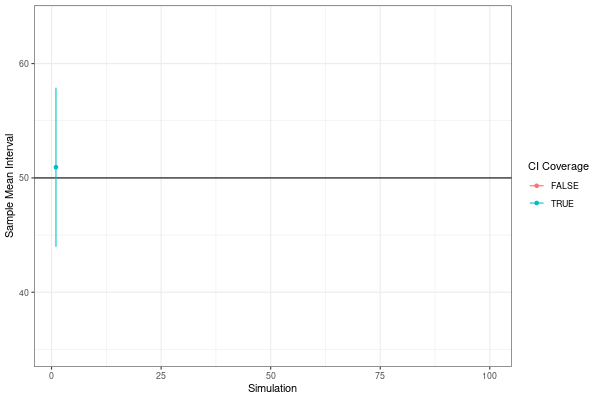
\includegraphics[scale=0.5]{cover1.png}
\end{center}
\end{frame}

\begin{frame}{Coverage}
\begin{center}
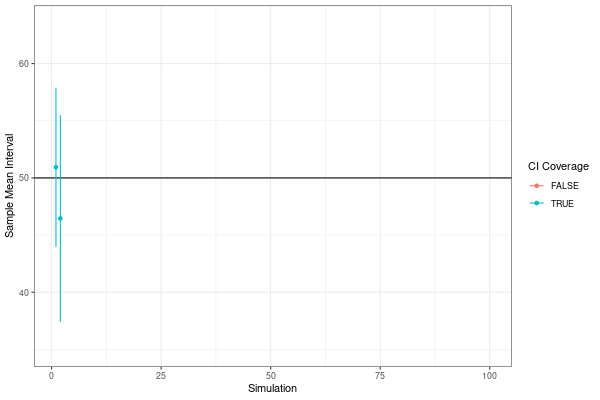
\includegraphics[scale=0.5]{cover2.png}
\end{center}
\end{frame}

\begin{frame}{Coverage}
\begin{center}
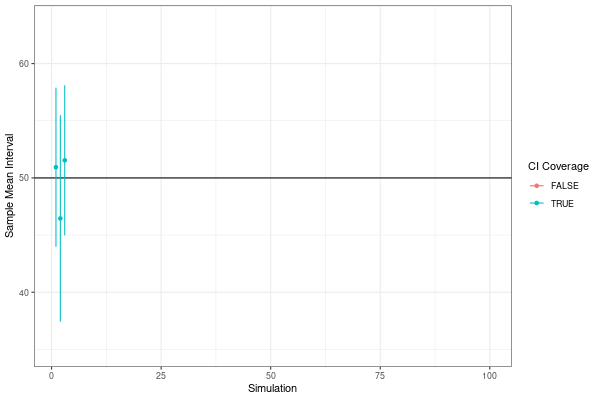
\includegraphics[scale=0.5]{cover3.png}
\end{center}
\end{frame}

\begin{frame}{Coverage}
\begin{center}
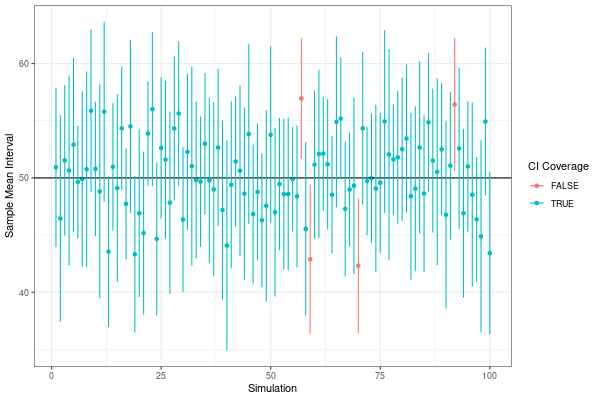
\includegraphics[scale=0.5]{cover4.png}
\end{center}
\end{frame}

\begin{frame}{Coverage}
\begin{center}
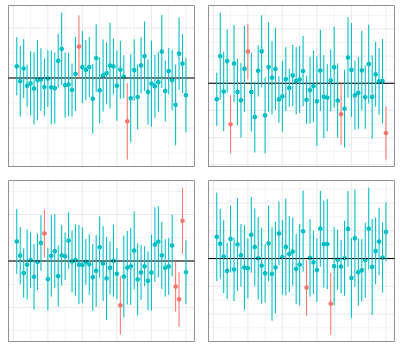
\includegraphics[scale=0.6]{all_ci100.png}
\end{center}
\end{frame}

\begin{frame}{Confidence Intervals}
To be absolutely clear: we will \textbf{never} know if the confidence interval we construct contains the true value of the parameter \vspace{8mm}

This is kind of like throwing a dart but never seeing the target \vspace{8mm}

This is the nature of statistical inference
\begin{itemize}
    \item we can describe properties of the \textit{process} that created our intervals
    \item we can never conclusively speak about the interval itself
\end{itemize}
\end{frame}


\begin{frame}{Confidence Intervals}
\footnotesize
It is also worth observing that we can \textit{alter} our process to achieve different results. There is a tradeoff between how frequently we are correct and how much uncertainty we allow in our prediction

\begin{center}
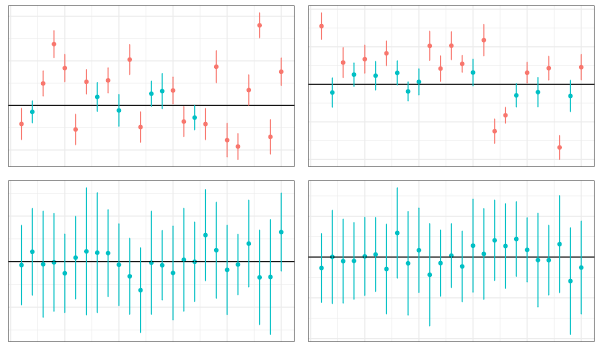
\includegraphics[scale=0.5]{diff_band.png}
\end{center}
\end{frame}

\begin{frame}{Common Misinterpretations}
These are some common ways people interpret CI's that are absolutely \textbf{not} correct: \vspace{2mm}
\begin{itemize}
    \item A 95\% confidence interval contains 95\% of the data in the population. \vspace{2mm}
    \item “I am 95\% sure that the mean of the sample will fall within a 95\% confidence interval for the mean.” \vspace{2mm}
    \item “95\% of all sample means will fall within this 95\% confidence interval.” \vspace{2mm}
    \item “The probability that the population parameter is in this particular 95\% confidence interval is 0.95.” \vspace{2mm}

\end{itemize}
\end{frame}

\begin{frame}{Generalizations}
Confidence Intervals quantify sampling variability
\begin{itemize}
    \item Range of plausible values for the statistic
    \item Range is determined by how much the statistics vary from sample to sample
\end{itemize} \vspace{8mm}

Confidence Intervals \textbf{DO NOT} account for bias in the samples
\begin{itemize}
    \item We will \underline{never} be able to quantify the bias in our samples
    \item It is important to mention possible sources of bias in our final conclusions
\end{itemize}
\end{frame}

%%%%%%%%%%%%%%%%

%\begin{frame}
%\begin{columns}
%
%  \begin{column}{0.45\textwidth}
%%
%  \end{column}
%  \begin{column}{0.45\textwidth}
%%
%  \end{column}
%
%\end{columns}
%\end{frame}


\end{document}
